%
% einleitung.tex -- Beispiel-File für die Einleitung
%
% (c) 2020 Prof Dr Andreas Müller, Hochschule Rapperswil
%
% !TEX root = ../../paper.tex
% !TEX encoding = UTF-8
%
\section{Geschichte\label{geostrophisch:section:geschichte}}
\kopfrechts{Geschichte}

Die Anfänge der numerischen Wettervorhersage gehen auf den britischen Mathematiker und Physiker \emph{Lewis Fry Richardson} (1881–1953) zurück (Abbildung~\ref{bild:portraitRichi}).
\index{Wettervorhersage}%
\index{numerische Wettervorhersage}%
Schon in jungen Jahren entdeckte er sein Interesse an der Mathematik und wie man diese einsetzen kann, um die Menschheit voranzubringen.
Er entwickelte eine neue spezielle Methode, um analytisch nicht lösbare partielle Differentialgleichungen zu lösen. 
Besagte Methode wurde in einem Artikel veröffentlicht.
Anschliessend forschte er an praktischen Anwendungsmöglichkeiten für seine entwickelte Methode.

In seinem Werk \cite{geostrophisch:wpbnp} formulierte Richardson bereits 1922 als Erster die Idee, eine numerische Wettervorhersage durch das explizite Lösen eines physikalisch fundierten Gleichungssystems zu bestimmen.  
Damit legte er den theoretischen Grundstein für die moderne Wettermodellierung.
\index{Wettermodellierung}%
Da er in diesem Buch ein praktisch gerechnetes Beispiel inkludieren wollte, führte er die Berechnung seiner Idee einmal praktisch durch.
Für diese erste Vorhersage von sechs Stunden brauchte er etwa sechs Wochen Zeit für die Berechnungen.
Doch seine erste Vorhersage wich sehr stark von der Realität ab.
Was dabei schief ging und wieso seine Arbeit doch so grundlegend wichtig für heutige Wettervorhersagen ist, wird in Abschnitt~\ref{geostrophisch:subsection:failedPrediction} genauer beschrieben.

Während Richardson das Buch \cite{geostrophisch:wpbnp} verfasste, war er als Krankenwagenfahrer im Krieg tätig. 
Obwohl er Pazifist war und nichts mit dem Krieg zu tun haben wollte, wurde er aufgefordert, seinen Teil beizutragen. 
Die atmosphärischen Daten für seine Berechnungen findet er in einem Bericht vom 20. Mai 1910. 
An diesem Tag war ein ``Internationaler Ballon-Tag'', in ganz Europa lies man Wetterballone aufsteigen, welche Daten der Atmosphäre sammelten.
\index{Wetterballon}%
\index{Ballon-Tag}%
Von dieser Messung um 7:00 Uhr wollte er das Wetter sechs Stunden vorhersagen. 
Nach Abschluss des Manuskripts lagerte Richardson es in einem Schuppen, in dem er auch Brennmaterial aufbewahrte.
So ging das Buch verloren und wurde erst Monate später unter einem Kohlehaufen wieder aufgefunden.
Diese Anekdote erwähnt er in zwei nüchternen Sätzen im Vorwort des Buches, dabei hätte es fast jahrelange Arbeit gekostet. 

Richardsons numerischer Ansatz war seiner Zeit voraus.
Das Buch war damals nicht in der Fachwelt anerkannt und wurde nicht viel verkauft. 
Seine Methode wurde als zu theoretisch und nicht umsetzbar betitelt. 
Sie erforderte enorme Rechenleistung, die damals nur durch Handberechnungen möglich war und daher für praktische Vorhersagen ungeeignet schien.  
Erst Jahrzehnte später, mit dem Aufkommen elektronischer Computer, konnte seine Methode effizient umgesetzt werden.  
\index{Computer}%
Die von ihm verwendeten Gleichungen, insbesondere in Verbindung mit der geostrophischen Näherung, bilden noch heute die Grundlage moderner Wettermodelle.

\begin{figure}[h]
	\centering
	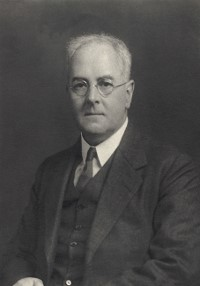
\includegraphics{Portrait_Richardson.jpg}
	\caption{Lewis Fry Richardson, 1881-1953, Autor des Buches \cite{geostrophisch:wpbnp} und damit Begründer der numerischer Wettervorhersage.}
	\label{bild:portraitRichi}
\end{figure}







